\documentclass[]{beamer} 
\setbeamerfont{all}{size=\large}
\setbeamerfont*{itemize/enumerate body}{size=\large}
\setbeamerfont*{itemize/enumerate subbody}{parent=itemize/enumerate body}
\setbeamerfont*{itemize/enumerate subsubbody}{parent=itemize/enumerate body}
\beamertemplatenavigationsymbolsempty
\usetheme{default}
\useinnertheme{circles}
\usebeamerfont{all}
\DeclareMathOperator*{\argmin}{arg\,min}
\usepackage{listings}
\usepackage{amssymb}
\usepackage{amsmath}
\usepackage{docmute}
\usepackage{hyperref}
\usepackage{multirow}
%\usepackage[export]{adjustbox}
\usepackage{graphicx}
\begin{document}

%\hspace*{\fill} \\

\title{In-network Upsampling with Convolutional Nets}
\author{Nicholas Dronen}


\begin{frame}
\maketitle
\end{frame}


\begin{frame}{Transposed Convolution (wrongly, ``Deconvolution'')}
\centering
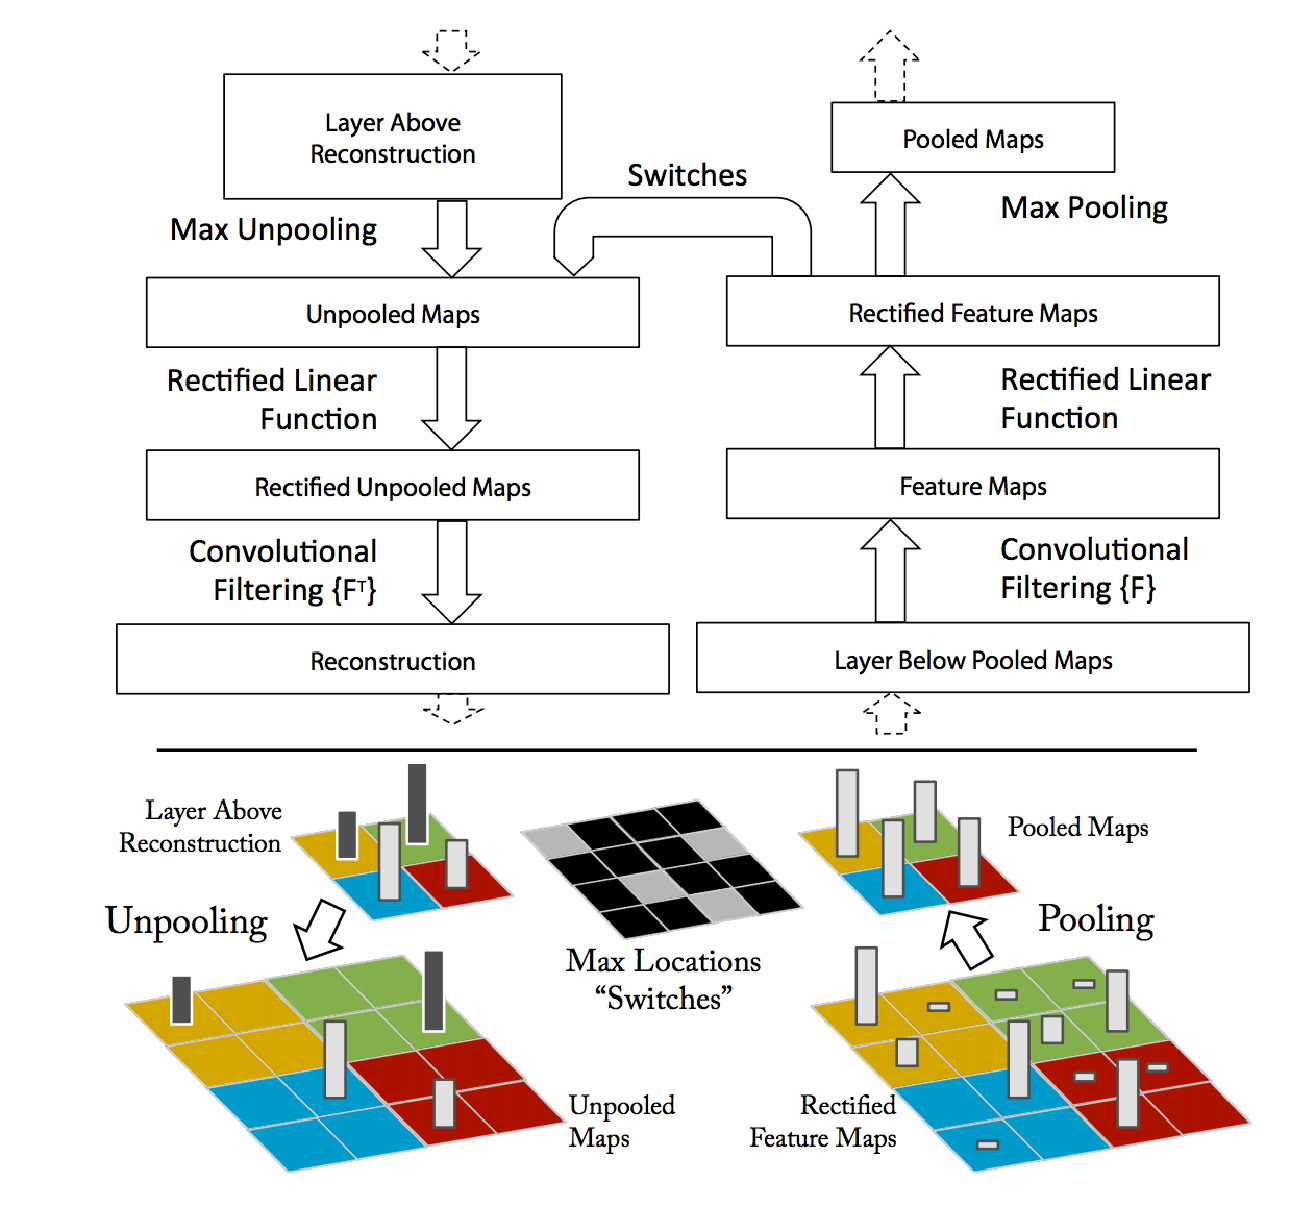
\includegraphics[width=0.75\textwidth]{figures/zeiler-transposed} \\
\href{https://arxiv.org/abs/1311.2901}
{\textcolor{blue}{Visualizing and Understanding Convolutional Networks, Zeiler and Fergus, arXiv:1311.2901 [cs.CV]}}
\end{frame}


\begin{frame}{Why ``Transposition''?}
Error is propagated back through e.g. a multi-layer perceptron via transposition of weight matrices. \\
\vspace{2mm}
\centering
On the forward pass for a layer $\ell$,
\begin{equation*}
z^{\ell} = \sigma(x\mathbf{M}_{\ell} + b_{\ell}).
\end{equation*}
Then, going backward, 
\centering
\begin{equation*}
\delta^{\ell} = \mathbf{M}^{\color{red}{T}} \delta^{\ell+1} \odot {z^{\ell}}^{\prime}.
\end{equation*}
\end{frame}


\begin{frame}{Transposition with 1d Convolutions}
Let $x \in R^{k \times 1}$ and $\mathbf{H} \in R^{d \times k}$ be a Toepliz matrix representation of a filter $h \in R^{k}$. \\
\vspace{2mm}
\centering
On the forward pass,
\begin{equation*}
y = \mathbf{H} x.
\end{equation*}
And going backward (assume $\mathbf{H}$ is orthogonal),
\begin{equation*}
x = \mathbf{H}^{\color{red}{T}} y.
\end{equation*}
\end{frame}


\begin{frame}{Discrete Convolution - 2d}
\centering
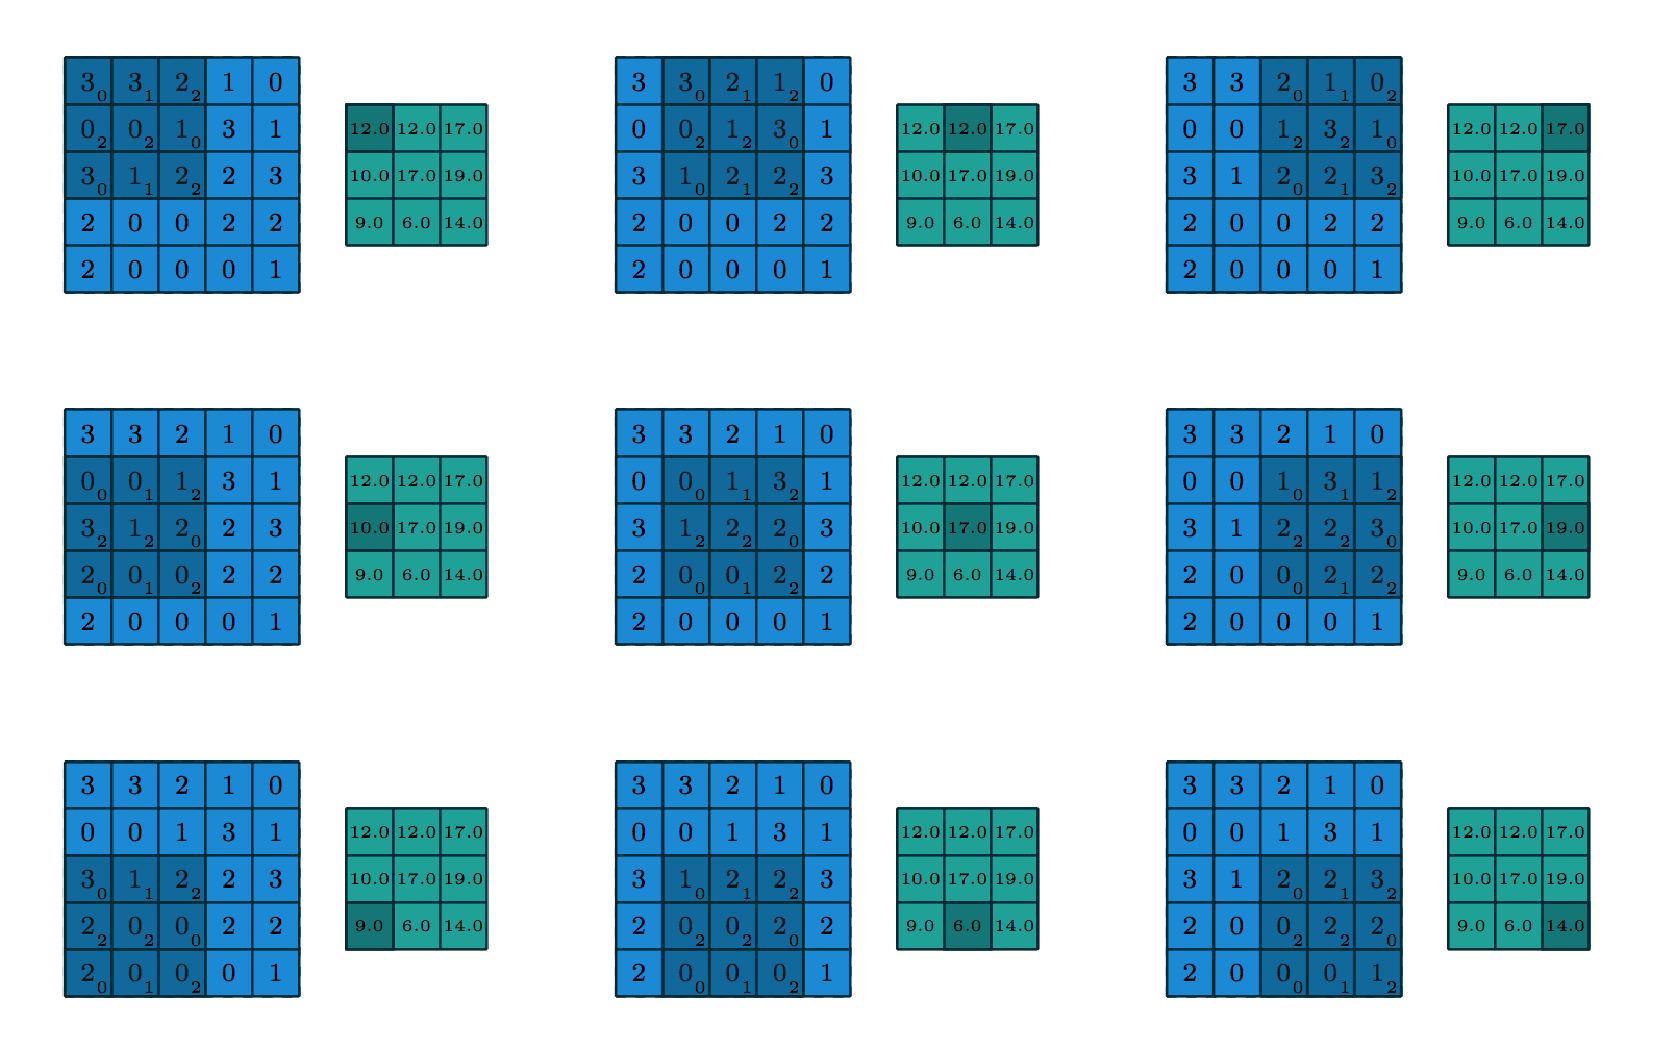
\includegraphics[scale=0.325]{figures/discrete-convolution} \\
\href{https://arxiv.org/abs/1511.07122}
{\textcolor{blue}{A guide to convolution arithmetic for deep learning, Dumoulin and Visin, arXiv:1603.07285 [stat.ML]}}
\end{frame}


\begin{frame}{Transposed Convolution - 2d}
\centering
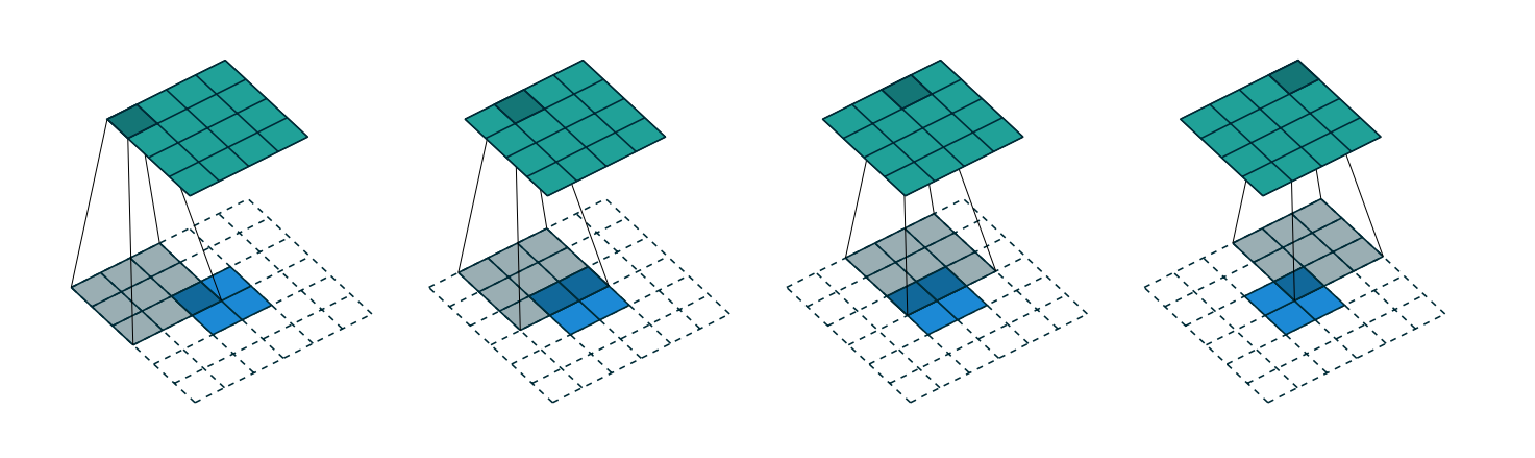
\includegraphics[scale=0.325]{figures/transposed-convolution} \\
\href{https://arxiv.org/abs/1511.07122}
{\textcolor{blue}{A guide to convolution arithmetic for deep learning, Dumoulin and Visin, arXiv:1603.07285 [stat.ML]}}
\end{frame}


\begin{frame}{Subpixel Convolution}
\centering
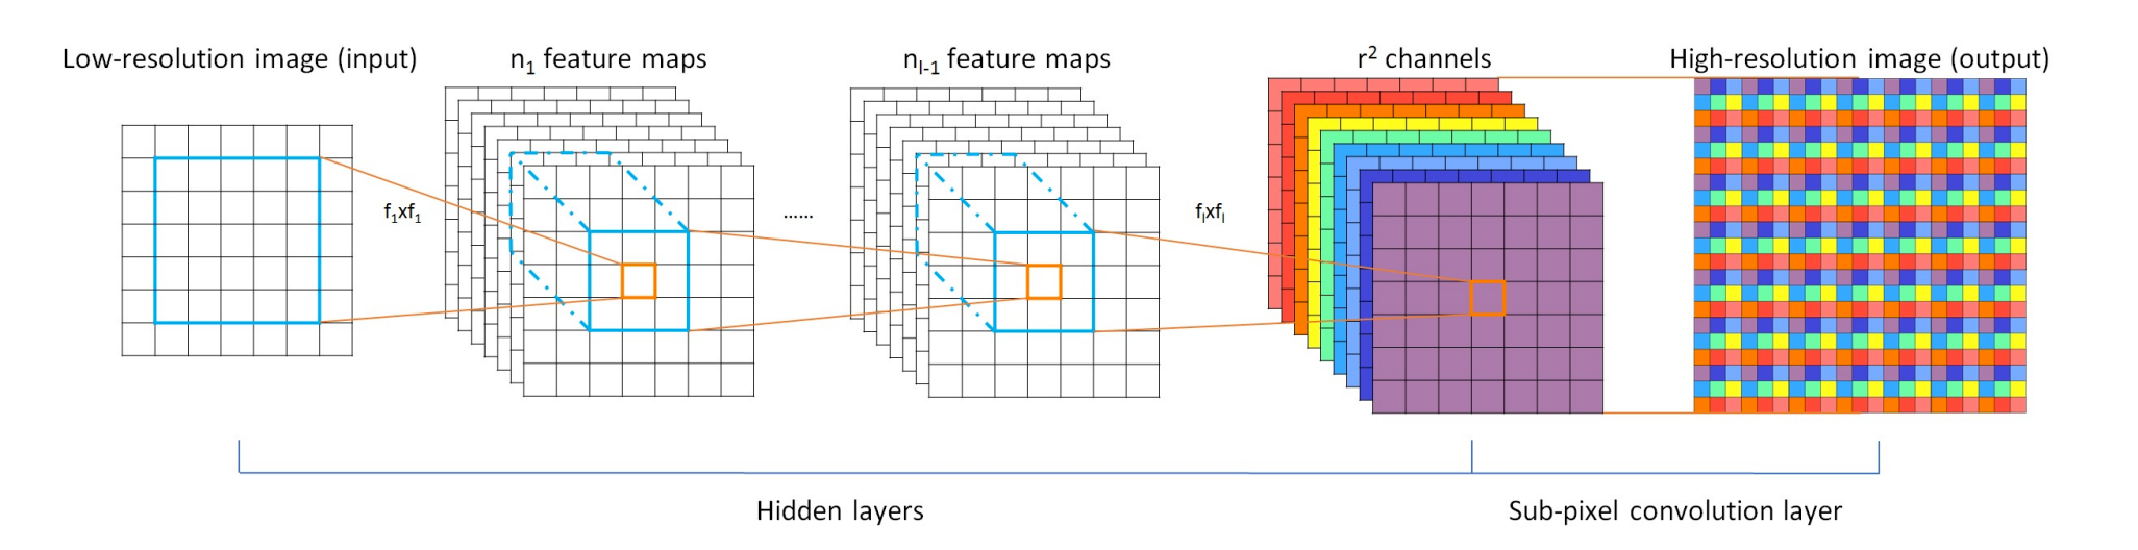
\includegraphics[width=0.85\textwidth]{figures/shi-subpixel} \\
\href{https://arxiv.org/abs/1609.05158}
{\textcolor{blue}{Real-Time Single Image and Video Super-Resolution Using an Efficient Sub-Pixel Convolutional Neural Network, Shi et al, arXiv:1609.05158 [cs.CV]}}
\end{frame}


\begin{frame}{Subpixel Convolution}
\centering
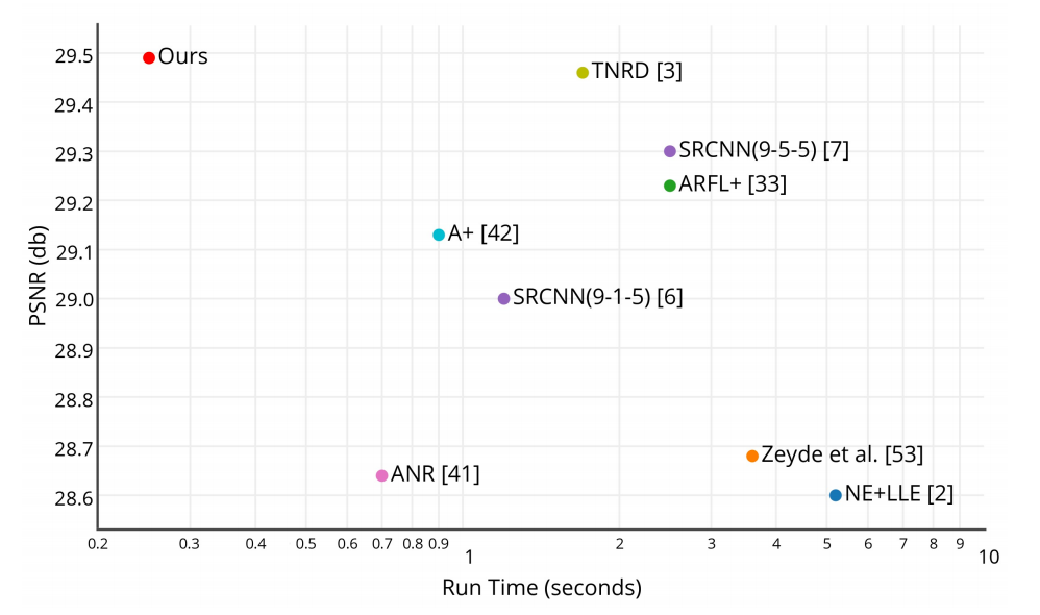
\includegraphics[width=0.85\textwidth]{figures/shi-subpixel-trade-off} \\
\href{https://arxiv.org/abs/1609.05158}
{\textcolor{blue}{Real-Time Single Image and Video Super-Resolution Using an Efficient Sub-Pixel Convolutional Neural Network, Shi et al, arXiv:1609.05158 [cs.CV]}}
\end{frame}


\begin{frame}{Transposed vs. Subpixel Convolutions}
\centering
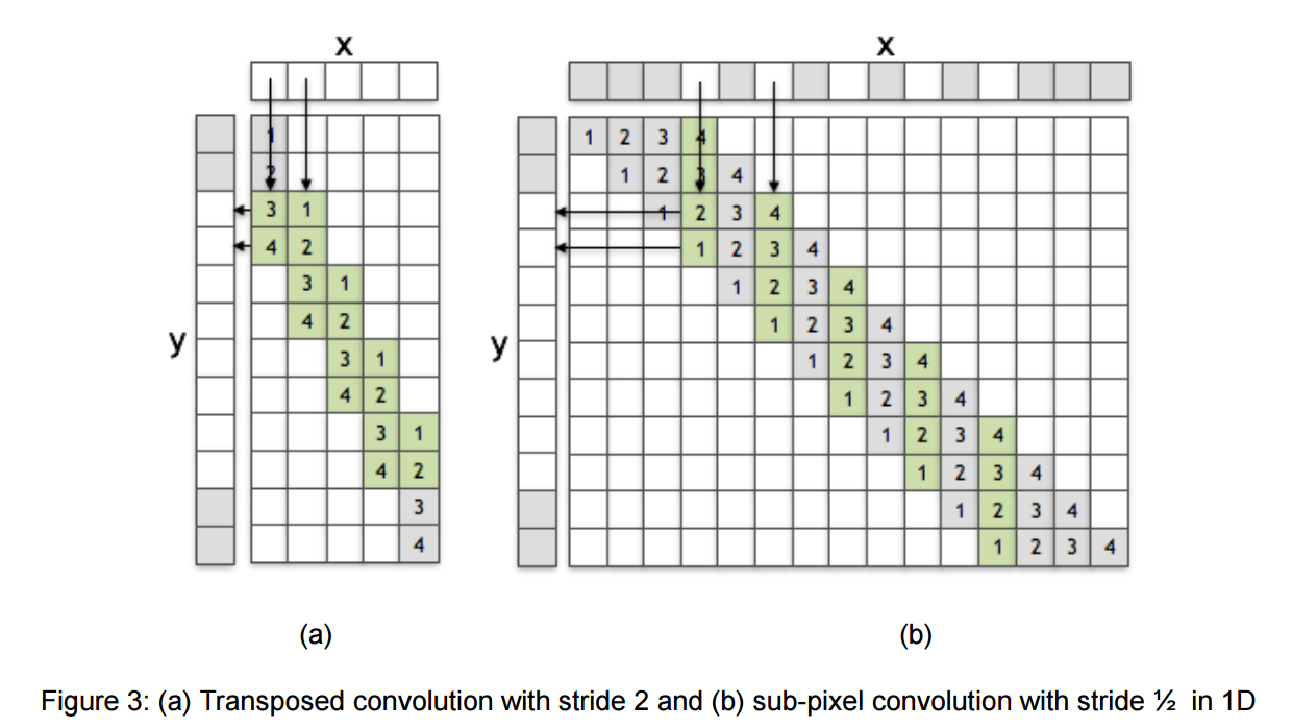
\includegraphics[width=0.85\textwidth]{figures/shi-subpixel-vs-transposed} \\
\href{https://arxiv.org/abs/1609.07009}
{\textcolor{blue}{Is the deconvolution layer the same as a convolutional layer?, Shi et al, arXiv:1609.07009 [cs.CV]}}
\end{frame}




\begin{frame}{Test bed: superresolution with drive images}
\centering
Upsampling from $60 \times 45 \rightarrow 480 \times 360$.
\begin{table}
\begin{tabular}{ccccc}
Resolution                           & NN Conv & BL Conv & SP Conv & XP Conv \\
\hline
\multirow{4}{*}{$120 \times 90$}     & NN      & BL      &         & \\
                                     & Conv    & Conv    & Conv    & XP Conv \\
                                     & PReLU   & PReLU   & PReLU   & PReLU \\
                                     &         &         & Shuffle & \\
\hline
\multirow{4}{*}{$240 \times 180$}    & NN      & BL      &         & \\
                                     & Conv    & Conv    & Conv    & XP Conv \\
                                     & PReLU   & PReLU   & PReLU   & PReLU \\
                                     &         &         & Shuffle & \\
\hline
\multirow{4}{*}{$480 \times 360$}    & NN      & BL      &         & \\
                                     & Conv    & Conv    & Conv    & XP Conv \\
                                     & PReLU   & PReLU   & PReLU   & PReLU \\
                                     &         &         & Shuffle & \\
\end{tabular}
\end{table}
\end{frame}


\begin{frame}{Upsampling without Training}
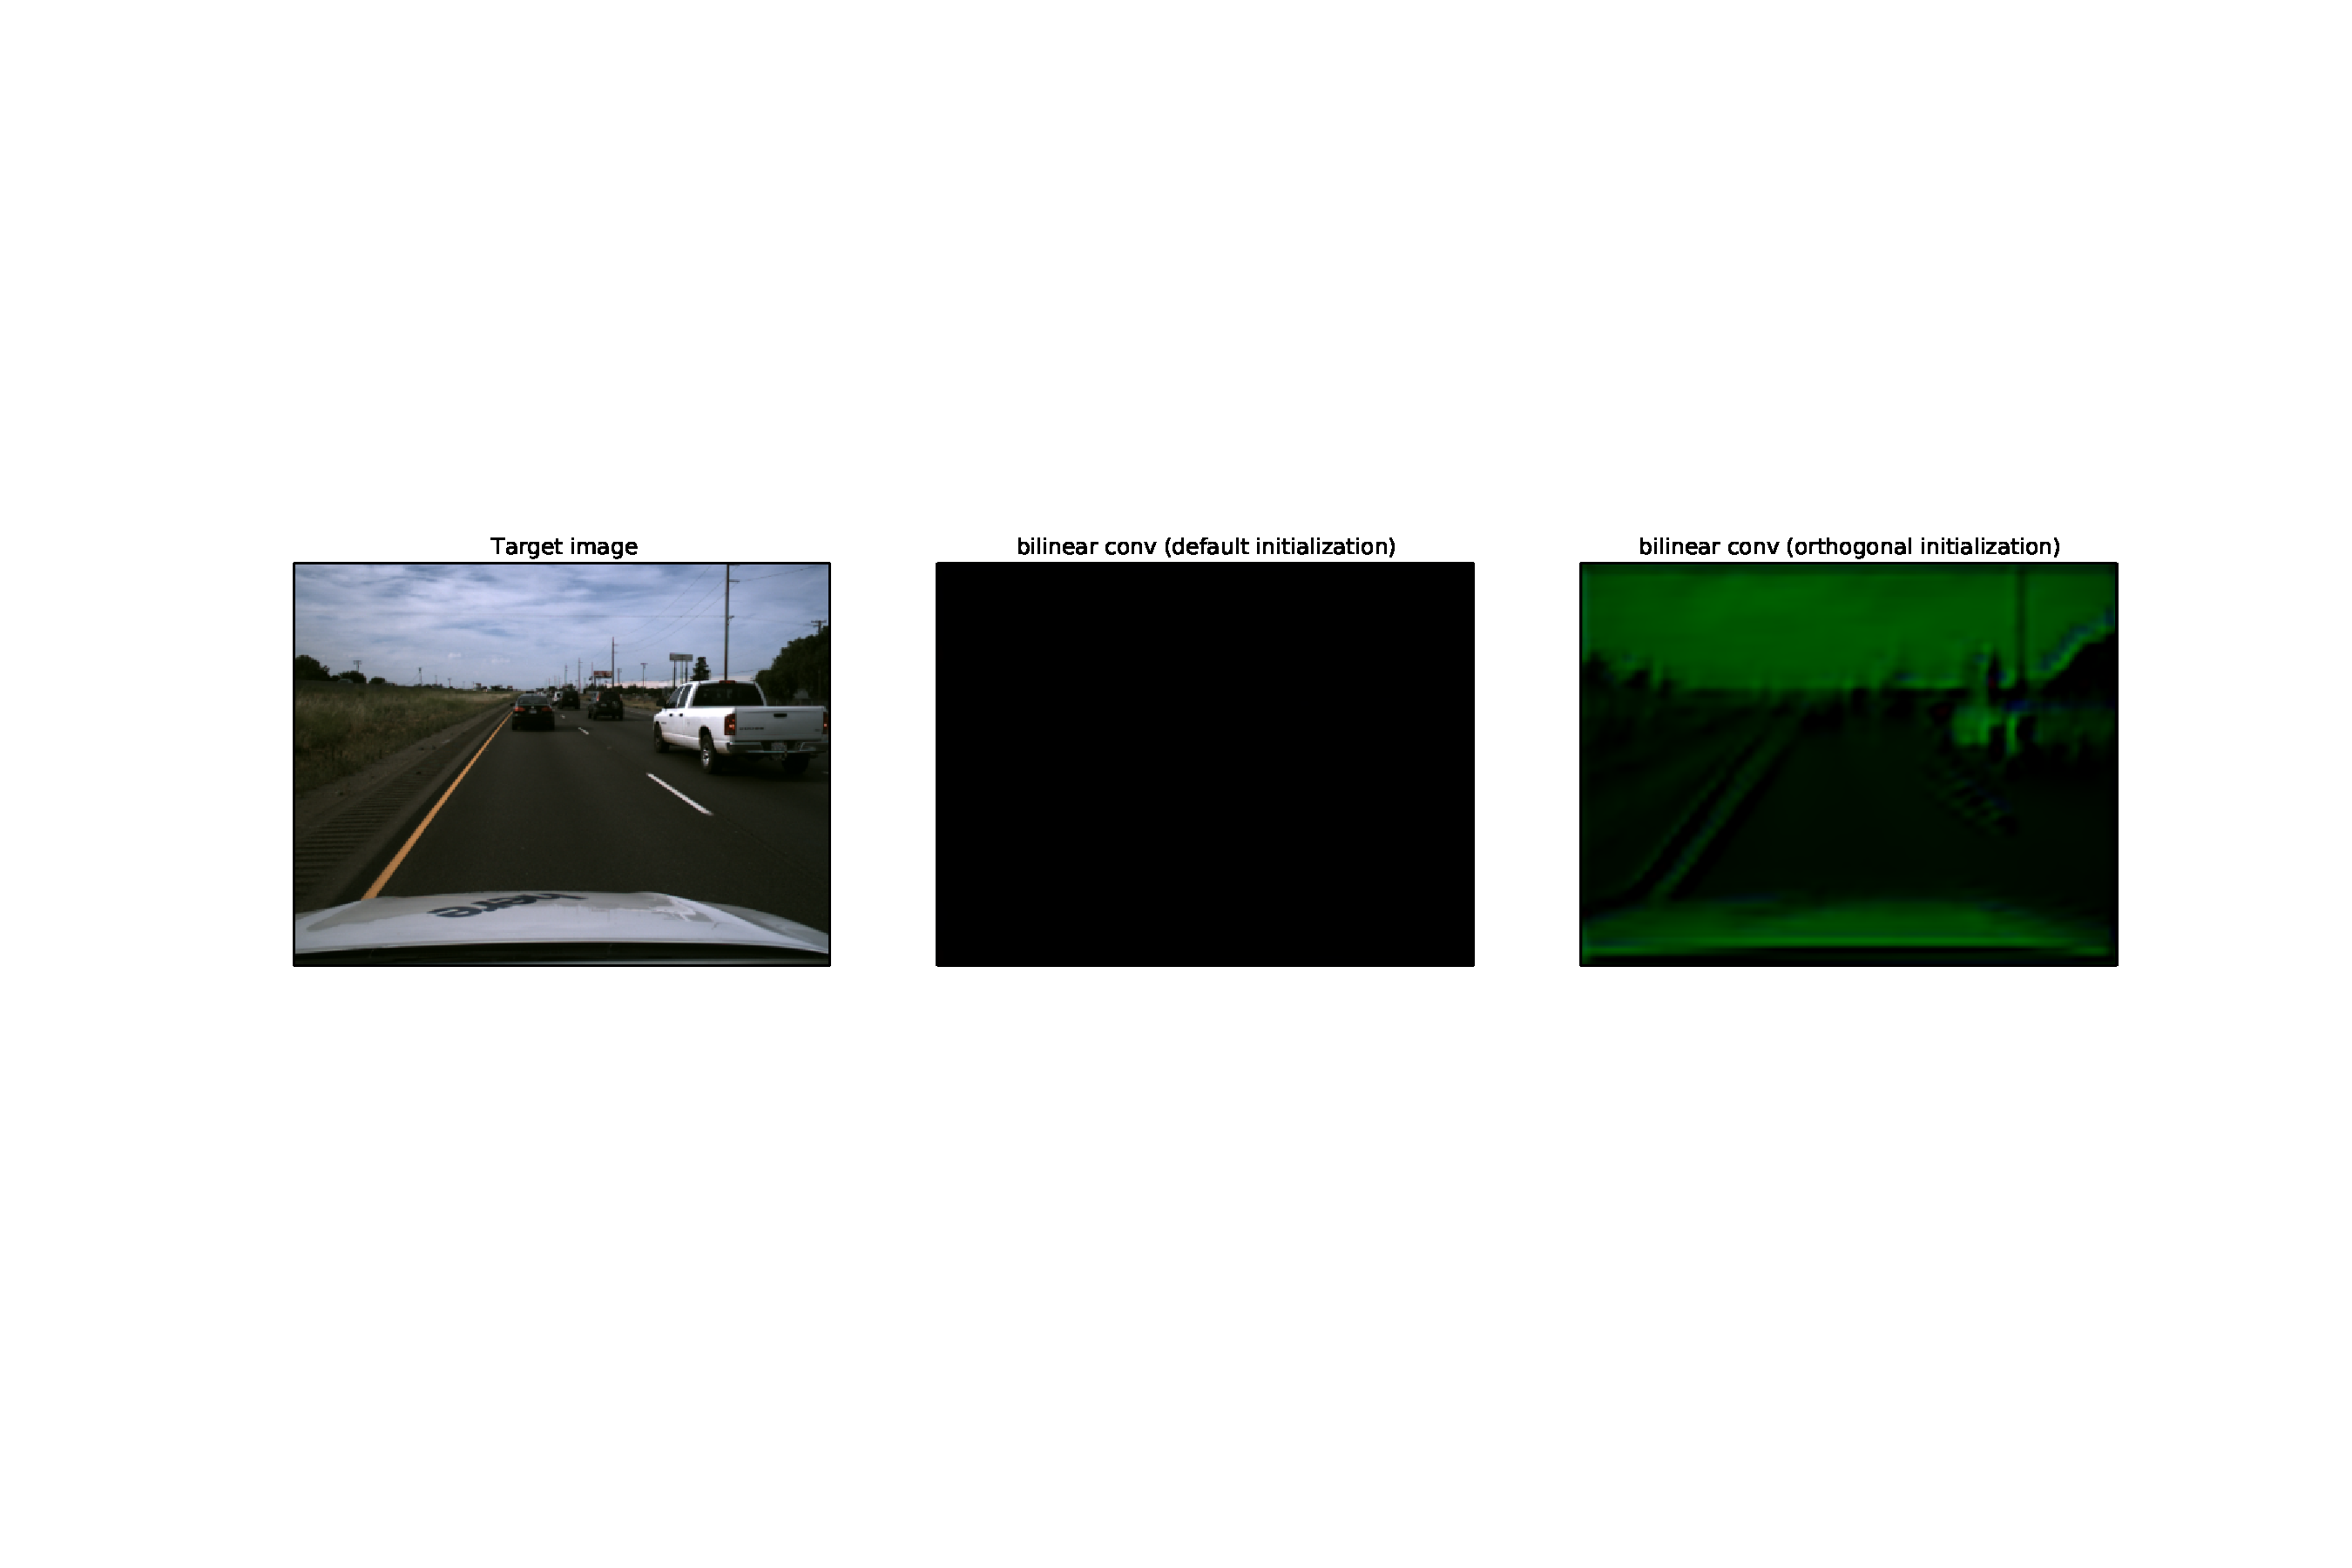
\includegraphics[width=1.0\textwidth, height=\textheight, trim={4cm 1cm 4cm 1cm},clip]{figures/bilinear-conv-initialization}
\end{frame}


\begin{frame}{Quantitative results - PSNR}
\begin{tabular}{lcccccc}
\hline
{PSNR} &  BL &  BL Conv &  NN &  NN Conv &  SP Conv &  XP Conv \\
\hline
Min         &  18 &       18 &  18 &       19 &             \textbf{20} &               18 \\
Max         &  25 &       27 &  26 &       \textbf{28} &             \textbf{28} &               26 \\
Mean        &  23 &       23 &  23 &       \textbf{25} &             \textbf{25} &               23 \\
%Std.        &   2 &        2 &   2 &        2 &              2 &                2 \\
%Median      &  23 &       23 &  23 &       25 &             \textbf{26} &               24 \\
N. Params   &   0 &      261 &   0 &      261 &           1044 &              261 \\
\hline
\end{tabular}
\end{frame}

\begin{frame}{Qualitative results}
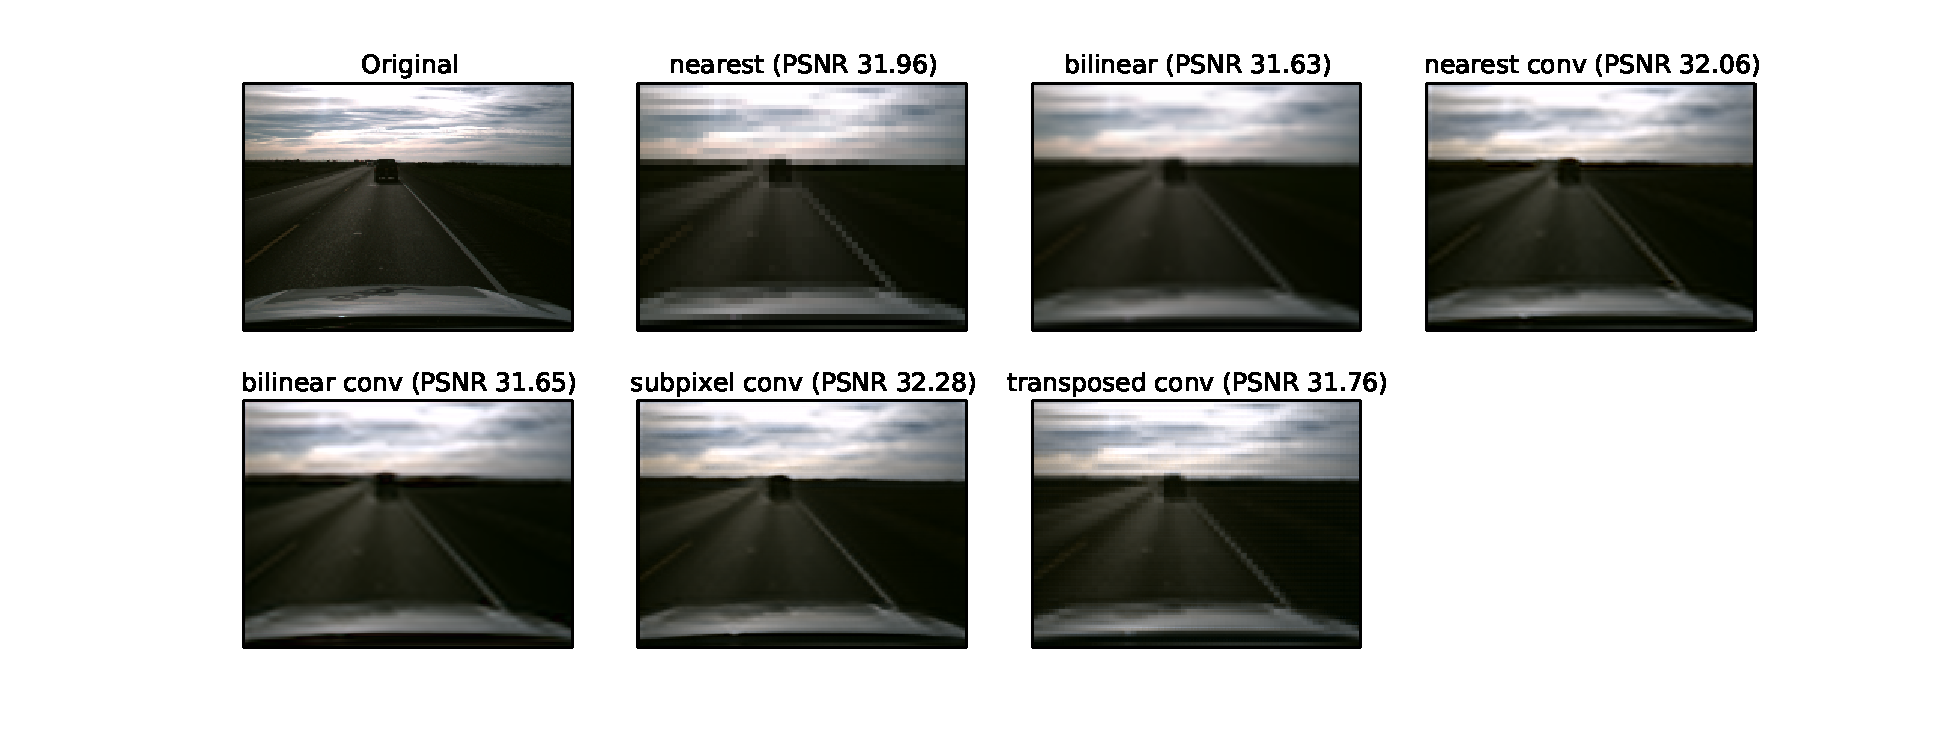
\includegraphics[width=1.0\textwidth]{figures/xposed-conv-highest-accuracy}
\end{frame}

\begin{frame}{Qualitative results}
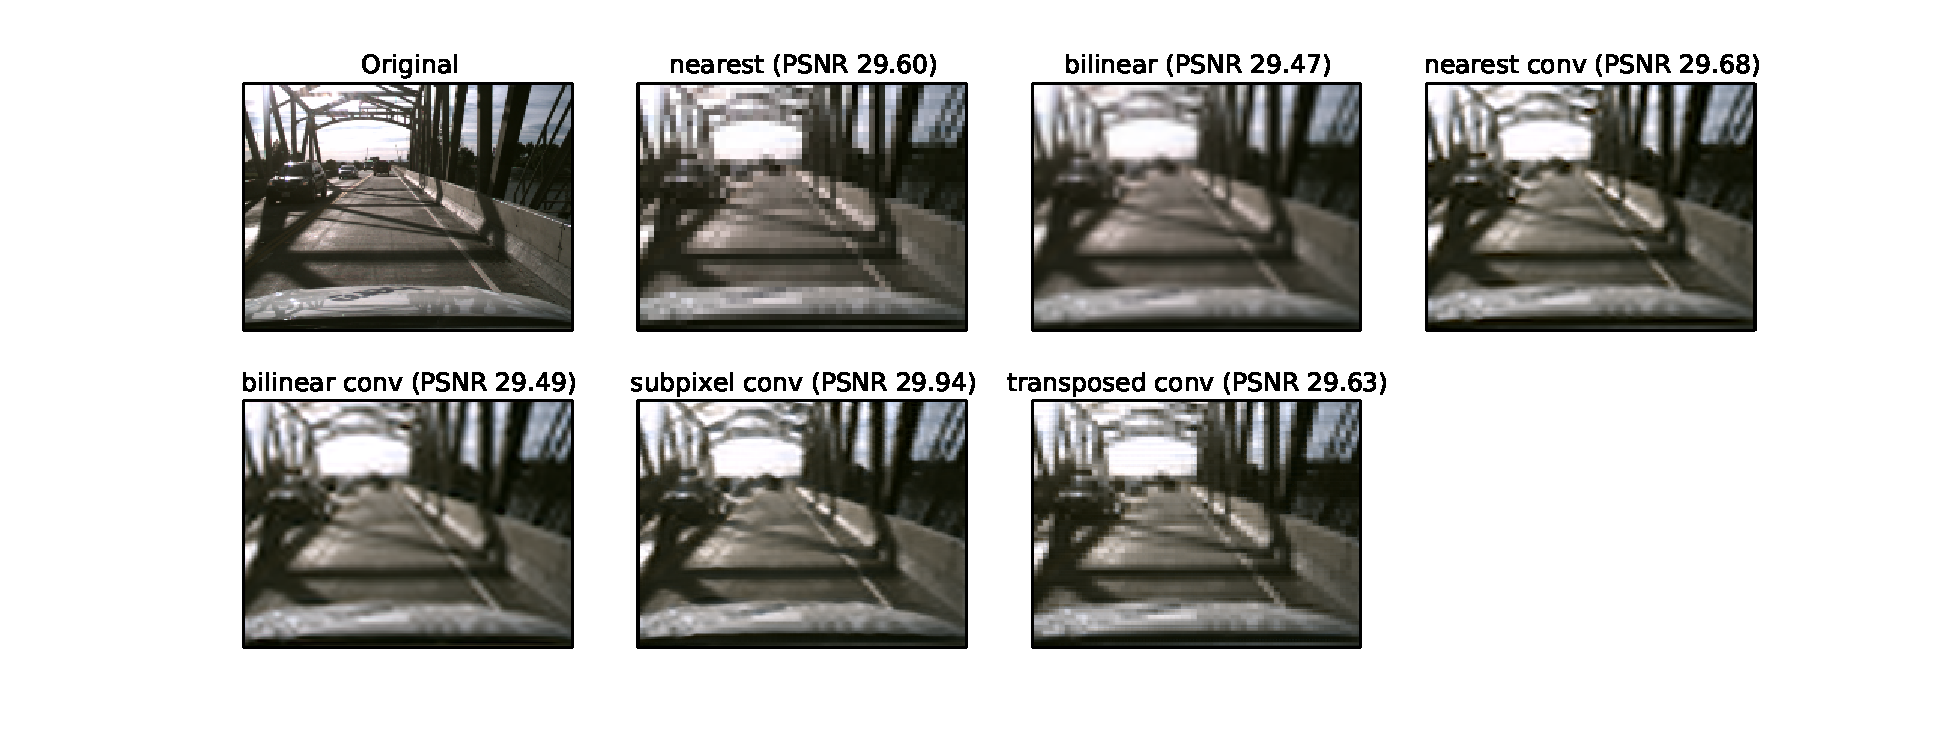
\includegraphics[width=1.0\textwidth]{figures/bilinear-conv-lowest-accuracy}
\end{frame}

\begin{frame}{Runtime performance}
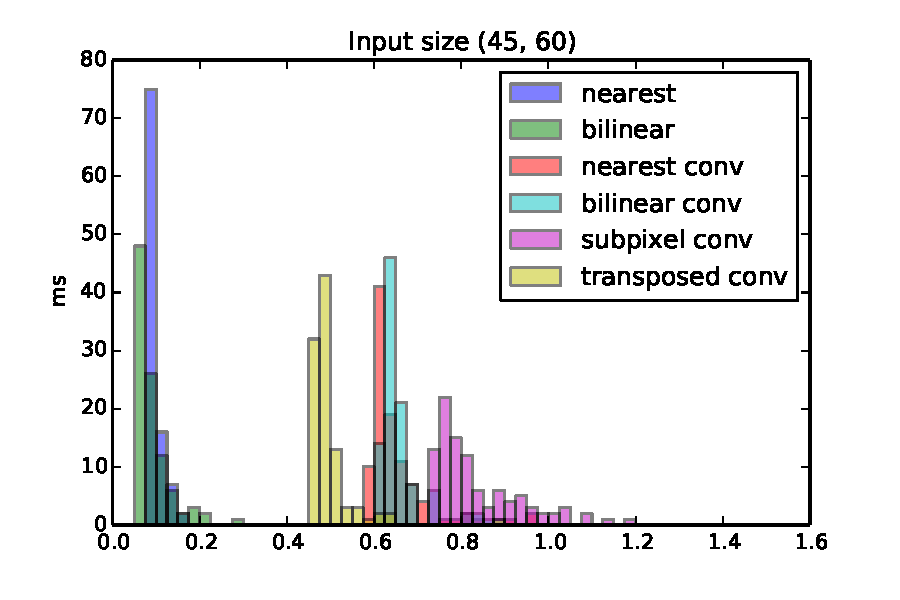
\includegraphics[width=1.0\textwidth]{figures/small-runtime-histogram}
\end{frame}

\begin{frame}{Error analysis}
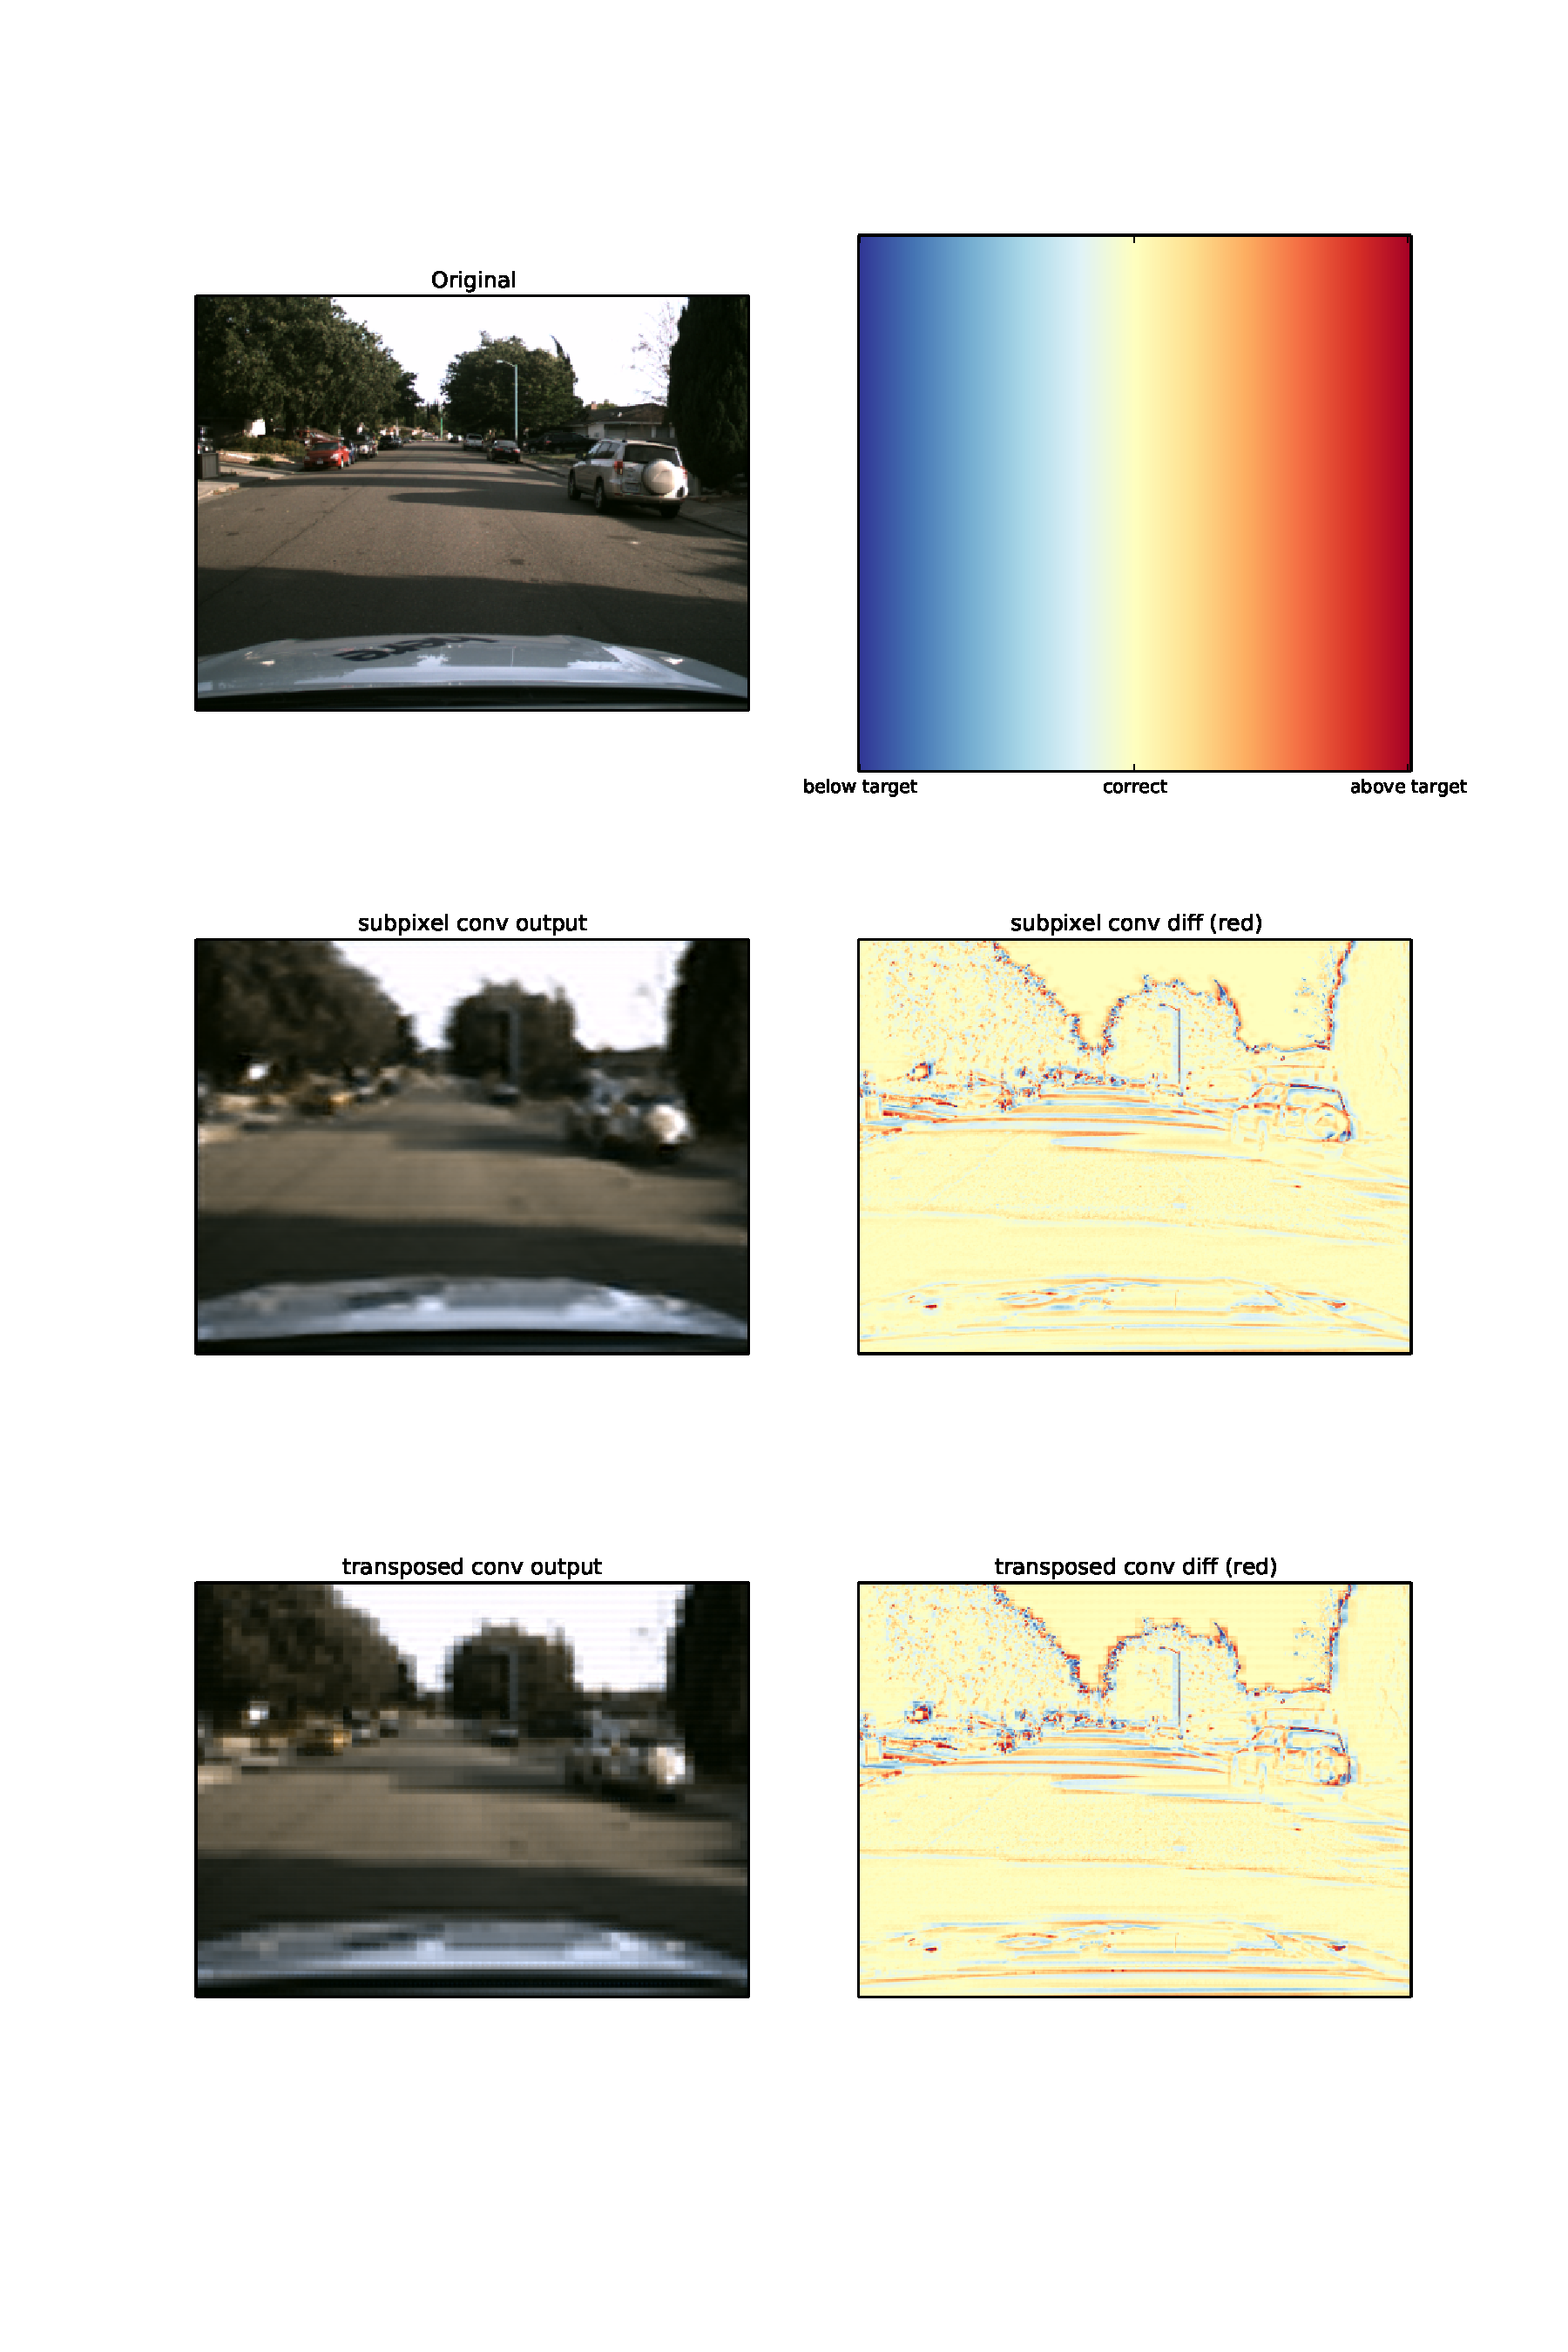
\includegraphics[height=1.0\textheight,width=1.0\textwidth]{figures/error-analysis}
\end{frame}

\end{document}
